% Created 2015-12-10 Thu 13:27
\documentclass{article}
\usepackage[top=1in, bottom=1.in, left=1in, right=1in]{geometry}
  \usepackage[makeroom]{cancel}
\usepackage{verbatim}


\usepackage[utf8]{inputenc}
\usepackage{lmodern}
\usepackage[T1]{fontenc}
\usepackage{fixltx2e}
\usepackage{graphicx}
\usepackage{longtable}
\usepackage{float}
\usepackage{wrapfig}
\usepackage{rotating}
\usepackage[normalem]{ulem}
\usepackage{amsmath}
\usepackage{textcomp}
\usepackage{marvosym}
\usepackage{wasysym}
\usepackage{amssymb}
\usepackage{amsmath}
\usepackage[version=3]{mhchem}
\usepackage[numbers,super,sort&compress]{natbib}
\usepackage{natmove}
\usepackage{url}
\usepackage{minted}
\usepackage{underscore}
\usepackage[linktocpage,pdfstartview=FitH,colorlinks,
linkcolor=blue,anchorcolor=blue,
citecolor=blue,filecolor=blue,menucolor=blue,urlcolor=blue]{hyperref}
\usepackage{attachfile}
\author{Abhishek Bagusetty}
\date{\today}
\title{24-623 2015 HM7}
\begin{document}

\maketitle

\section{Problem 1}
\label{sec-1}
\subsection{a)}
\label{sec-1-1}
\begin{figure}[htb]
\centering
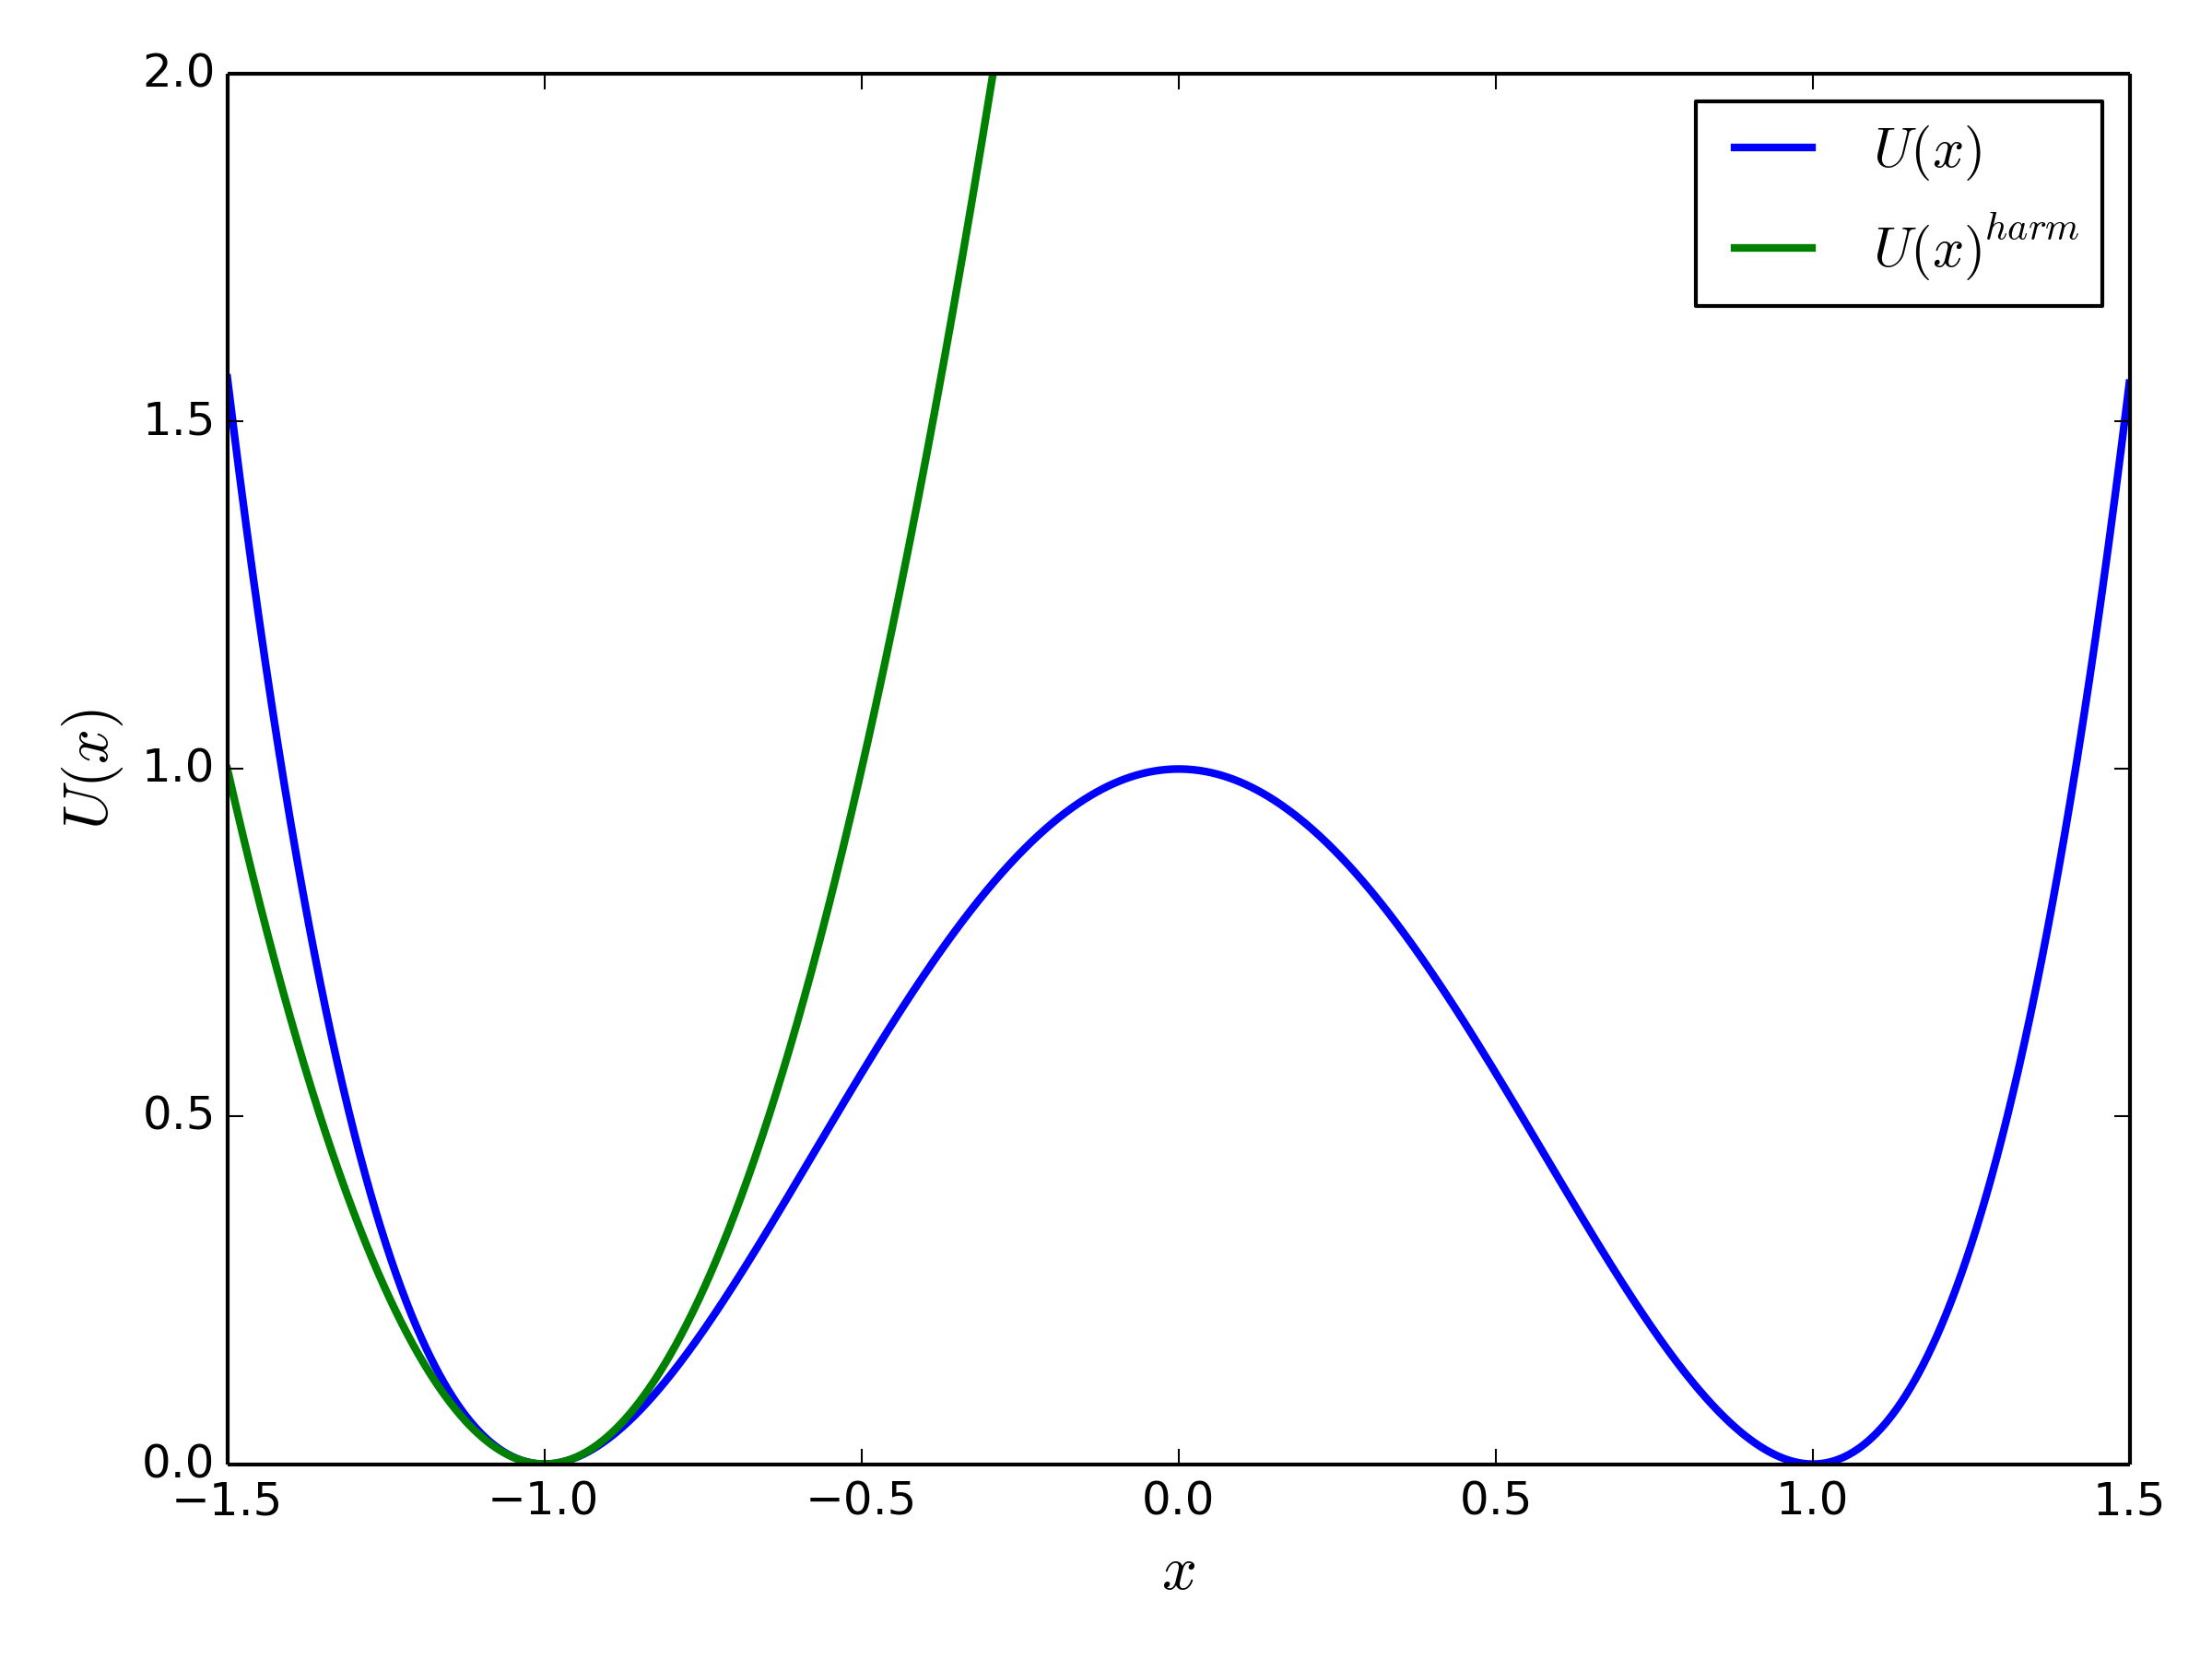
\includegraphics[width=.9\linewidth]{./P1/P1-a.png}
\caption{\label{fig:P1-a}The figure shows the plot of U(x) and its harmonic approximation in well A.}
\end{figure}

\subsection{b)}
\label{sec-1-2}
\begin{figure}[htb]
\centering
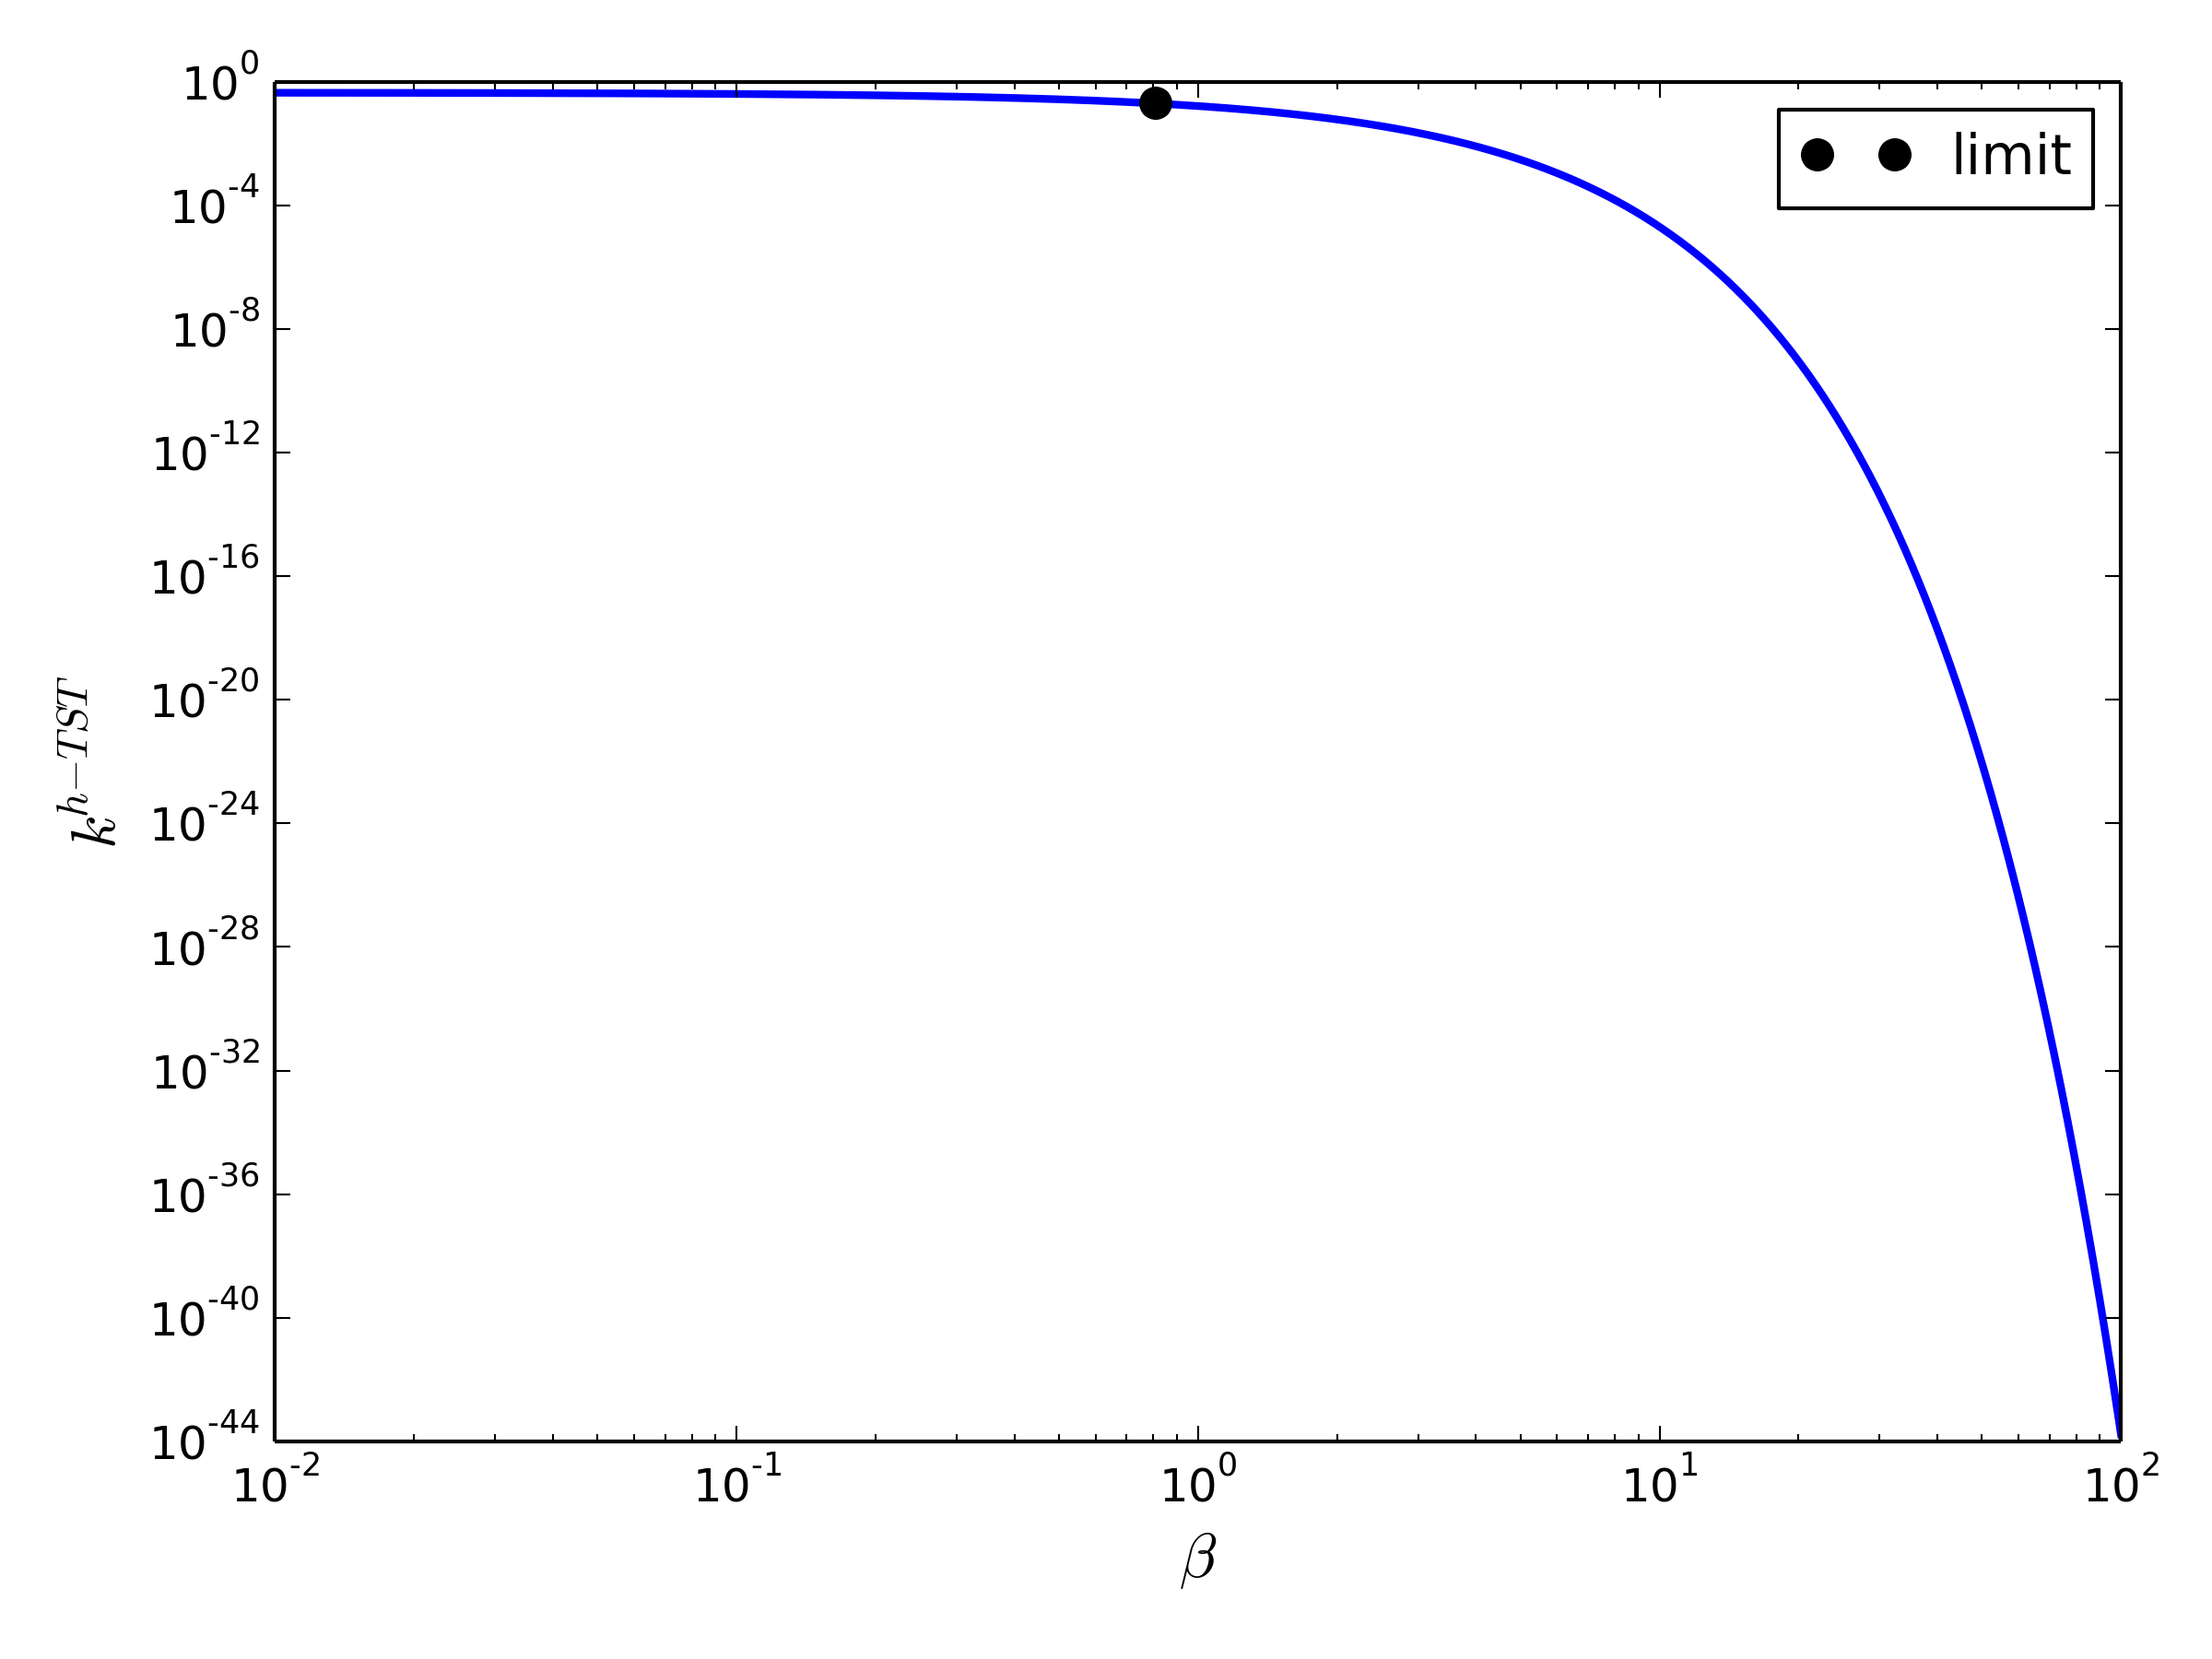
\includegraphics[width=.9\linewidth]{./P1/P1-b.png}
\caption{\label{fig:P1-b}The figure shows the plot of TST rate expression from harmonic approximation as a function of $\beta$.}
\end{figure}
The loglog plot of k$_{\text{A }\rightarrow\ \text{B}}^{\text{TST}}$ from the harmonic rate expression for a range of $\beta$ in Fig.\ref{fig:P1-b}.
\subsection{c)}
\label{sec-1-3}
Limit of the approximation is plotted in the Fig.\ref{fig:P1-b}. Value of k in the expression of harmonic TST rate is obtained by $\frac{d^2U(x)}{dx^2}$ at x$_{\text{o}}$. 

As the parameters $\beta$, k, q increases, the immediate consequence is the effect of having a value of the limit greater than 1.8. Higher the value of q would implies that minima and maxima are seperated to a greater extent. The value of k is related to $\frac{d^2U(x)}{dx^2}$ at x$_{\text{o}}$, which means that higher the value means the potential surface is concave upward. Concave upward in this context means that the local minima is driving towards a maximum indicated by the slope. All these variables drive towards predicting a better rate from harmonic transition state.

\section{Problem 2}
\label{sec-2}
\subsection{a)}
\label{sec-2-1}
\begin{figure}[htb]
\centering
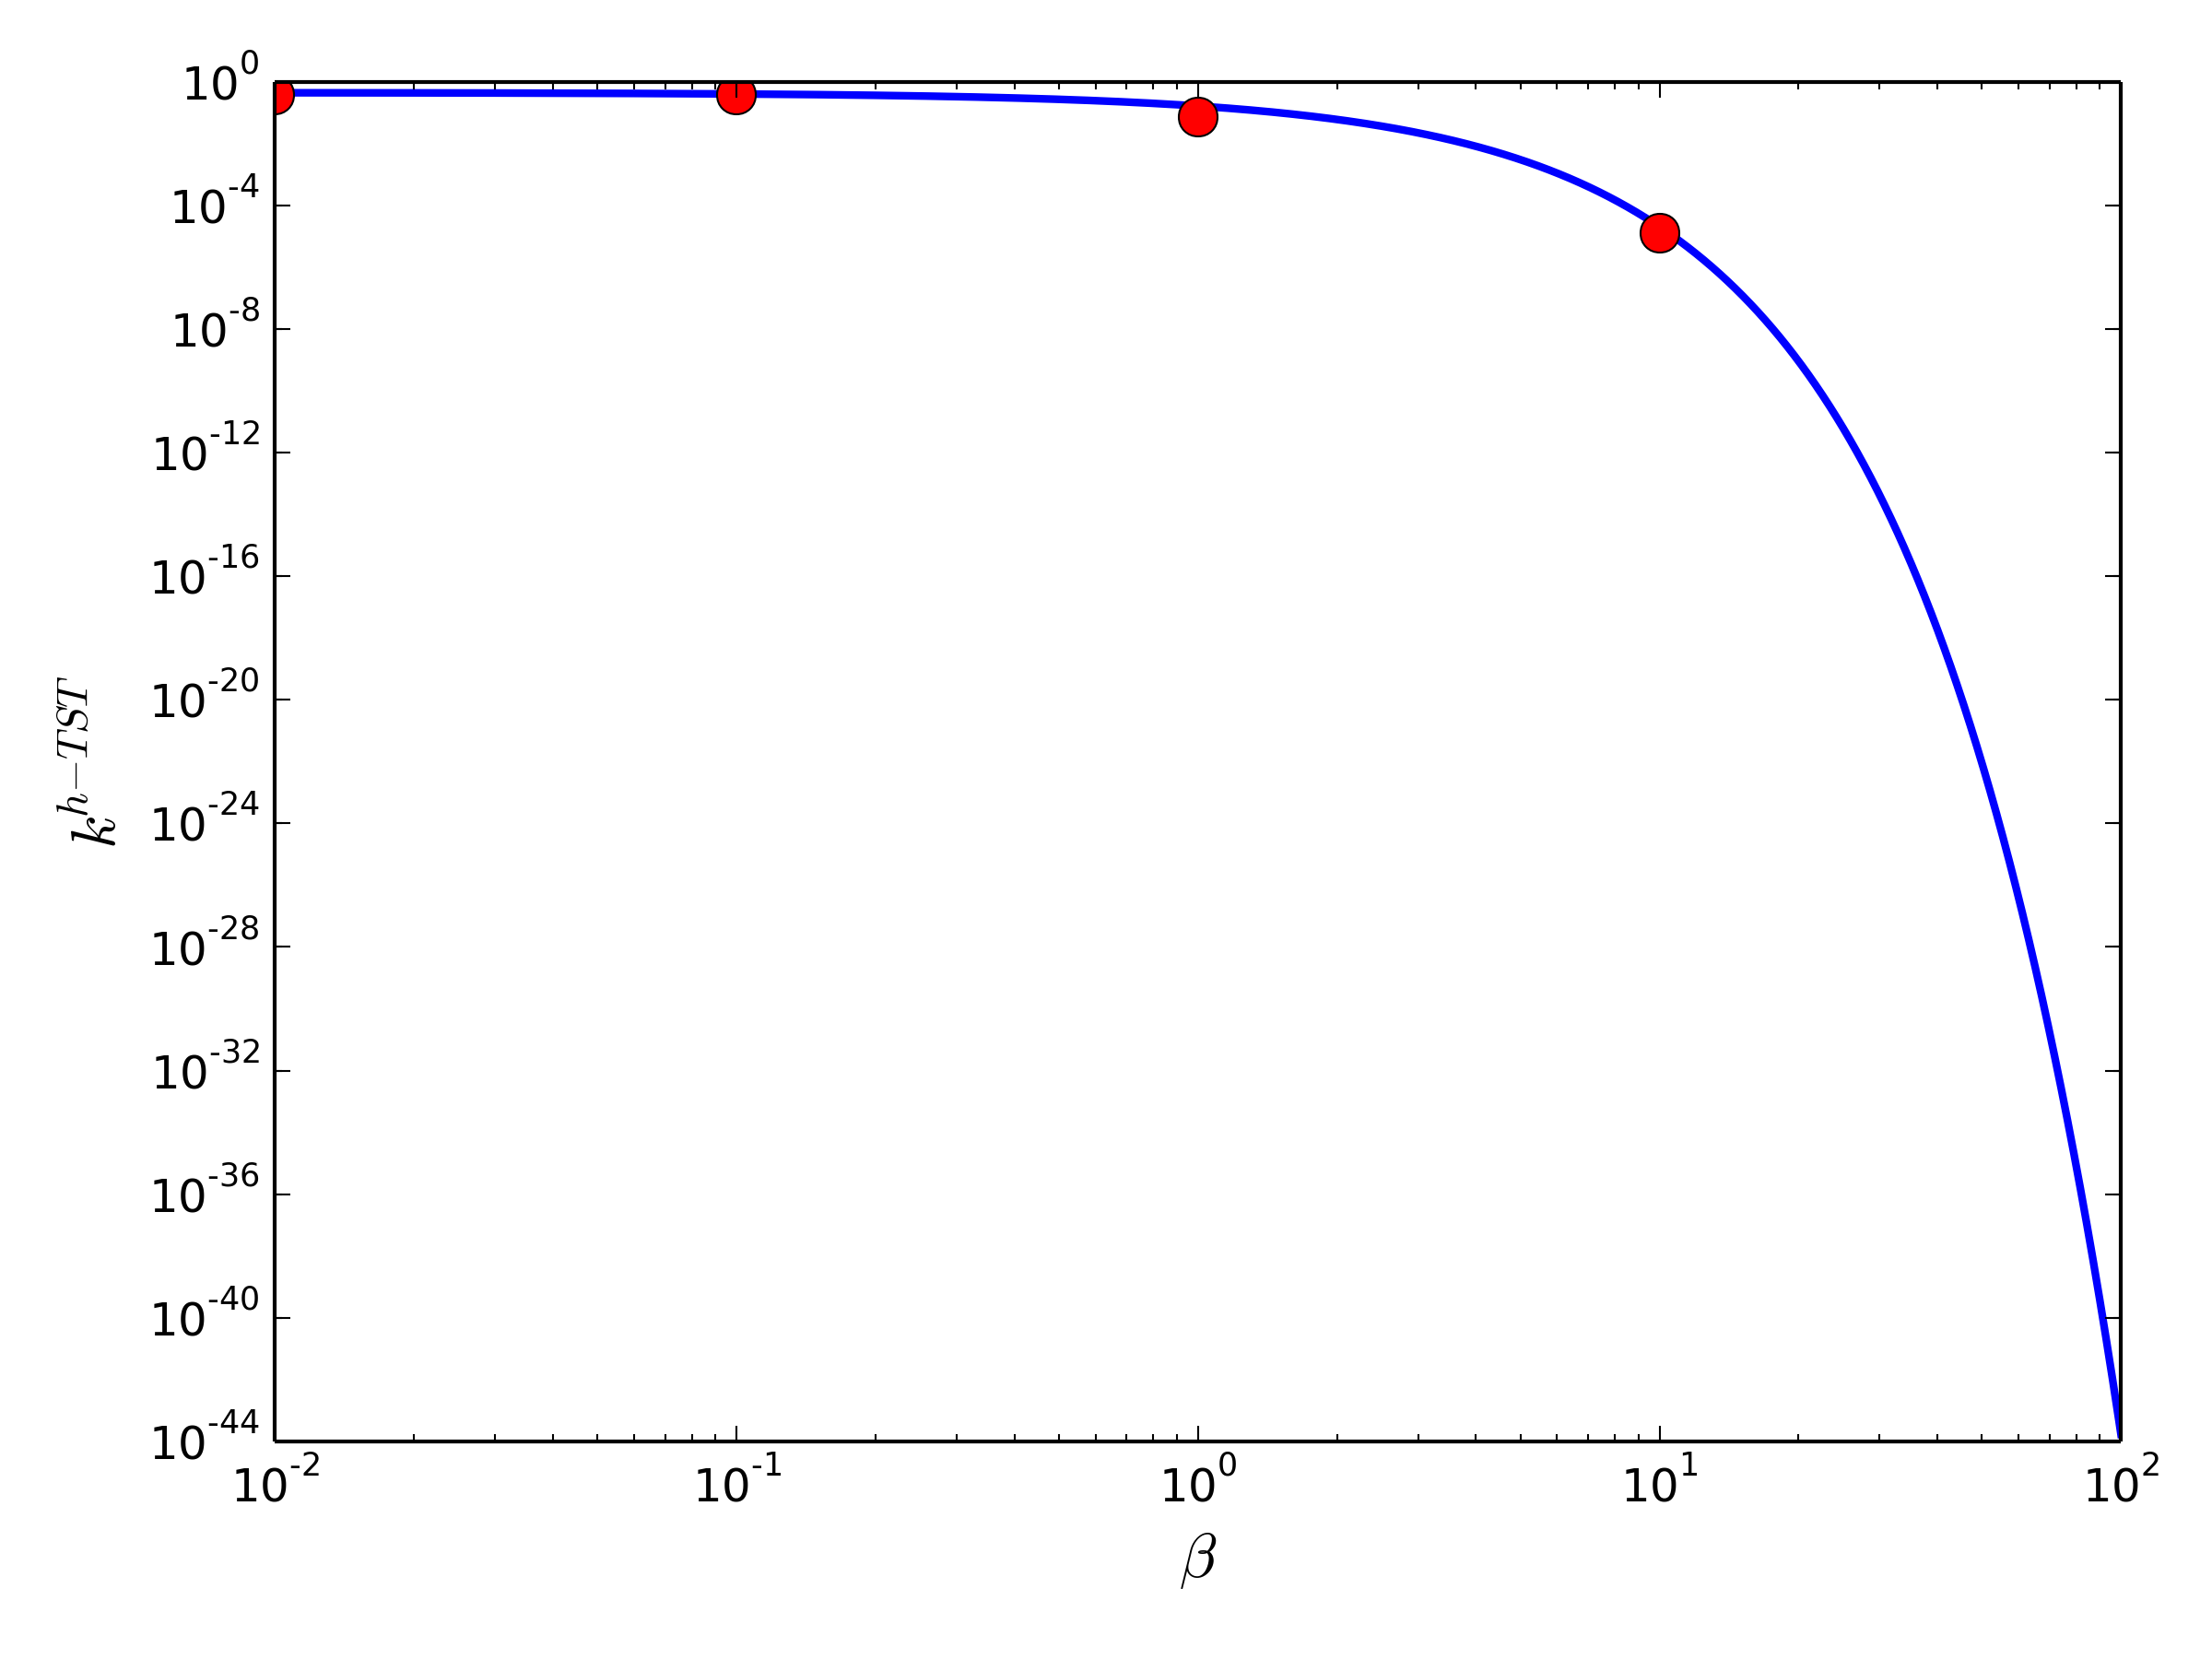
\includegraphics[width=.9\linewidth]{./P2/P1-b.png}
\caption{\label{fig:P2}The figure shows the plot of TST rate compute using the harmonic approximation and Metropolis NVT MC simulation}
\end{figure}

The values of the TST rate at different values of $\beta$ are tabulated from the harmonic approximation and Mertopolis NVT MC simualtion.
\begin{table}[htb]
\caption{TST rates from harmonic and MC techniques.}
\centering
\begin{tabular}{rrr}
$\beta$ & K\_HTST & K\_MC\\
\hline
0.01 & 0.445679 & 0.394075\\
0.1 & 0.4073199 & 0.376149\\
1 & 0.1656039 & 0.07155430\\
10 & 2.0437\,(-5) & 1.26157\,(-05)\\
100 & 1.6746\,(-44) & 0\\
\end{tabular}
\end{table}

\subsubsection{Computational Setup}
\label{sec-2-1-1}
Number of trial moves (N) is choosen sufficiently such that it is independent of other parameters in the simulation. The number of trial moves is chosen to be 10,000,000. With the N being kept constant, the $\epsilon$ value is chosen to be small enough that it would yeild an appropriate value of rate and the value is validated with the harmonic approximation. It is found that $\epsilon$ value of 0.005 yields a value converging well to harmonic approximation as shown in \ref{fig:P2}. With the above parameters kept constant, maximum step size is determined. Various values of maximum step size ranging from 0.01, 0.05, 0.1, 0.5, 5 for each value of $\beta$=[0.01, 0.1, 1, 10, 100].

\begin{table}[htb]
\caption{TST rates from harmonic and MC techniques at various maximum step sizes and at various values of $\beta$.}
\centering
\begin{tabular}{rrlrrrr}
$\beta$ & K\_HTST & K\_MC $\rightarrow$ &  &  &  & \\
\hline
dx$_{\text{max}}$ $\rightarrow$ &  & 0.01 & 0.05 & 0.1 & 0.5 & 5\\
0.01 & 0.445679 & 1.23975 & 1.03988 & 1.01451 & 0.986504 & \textbf{0.394075}\\
0.1 & 0.4073199 & \textbf{0.376149} & 0.31905 & 0.31191 & 0.305047 & 0.123129\\
1 & 0.1656039 & \textbf{0.0715543} & 0.0611977 & 0.0569291 & 0.0582216 & 0.0225402\\
10 & 2.0437\,(-5) & \textbf{1.26157E-05} & 1.76619\,(-05) & 1.26157\,(-05) & 7.5694\,(-06) & 0\\
100 & 1.6746\,(-44) & - & - & - & - & -\\
\end{tabular}
\end{table}

Vlaues highlighted in bold are the values converging to harmonic approximation benchmark. It is determined from the above table that dx$_{\text{max}}$ value of 0.01 yields good results with a resonable convergence to haromic approximation for the $\beta$ values of 0.1, 1, 10, 100. Maximum step size of 5 is used for the $\beta$=0.01.
Optimum value of $\epsilon$ is chosen based on its convergence to the value from harmonic approximation.

\begin{table}[htb]
\caption{TST rates from harmonic and MC techniques at various $\epsilon$ and at a fixed maximum step size and number of trial moves.}
\centering
\begin{tabular}{rrrrrr}
$\beta$ & K\_HTST & K\_MC $\rightarrow$ &  &  & \\
\hline
$\epsilon$ $\rightarrow$ &  & 0.01 & 0.05 & 0.1 & 0.005\\
0.01 & 0.445679 & 0.197157 & 0.0397267 & 0.0197716 & 0.394075\\
0.1 & 0.4073199 & 0.189412 & 0.03818 & 0.0186081 & 0.376149\\
1 & 0.1656039 & 0.03622 & 0.00716899 & 0.00360923 & 0.0715543\\
10 & 2.0437\,(-5) & 2.523\,(-06) & 1.00925\,(-06) & 7.567\,(-07) & 1.26157\,(-05)\\
100 & 1.6746\,(-44) & - & - & - & -\\
\end{tabular}
\end{table}

\subsection{b)}
\label{sec-2-2}
The rate obtained from monte carlo technique is greatly dependent on the following parameters - M, N and $\epsilon$. The rates obtained from both the techniques is comparable atleast with an order of magnitude. The rates computed from the MC-NVT-TST seems to be diverging from the harmonic approximations as the $\beta$ is getting higher and computations are not feasible as the temperature gets lower. 

The overall significance of relating rates to $\beta$ is interesting. At higher temperatures, one would have higher rates because the process is activated from thermal energy due the higher temperature (lower $\beta$).
The vibrational frequency at higher temperatures would increase for the bonds and hence the rates to drive the process would be higher. This process is vice-versa to that at the lower temperatures (higher $\beta$) as the frequency of vibration of bonds are not significant. This process is shown in Fig.\ref{fig:P2}
% Emacs 24.5.1 (Org mode 8.2.10)
\end{document}